\section{Principal Component Analysis}

\begin{enumerate}[label=\alph*), leftmargin=*]
%% a)
\item
%

The singular values of $\mathbf{X}$ and $\mathbf{X}_{noise}$ as well as their squared error between each singular value
are depicted in figure \ref{fig:2_3_a}.

The noiseless input matrix, $\mathbf{X}$, has 3 non-zero singular values, which reflect its rank.
The noise corrupted matrix, $\mathbf{X}_{noise}$, has 3 dominant singular values, corresponding to the eigenvectors spanning
the signal subspace, while the rest non-zero singular values correspond to the noise subspace. Moreover, the signal subspace
singular values are offset from the true singular values of $\mathbf{X}$, due to the noise corruption.

The noise subspace eigenvalues are half the magnitude compared to the signal subspace eigenvalues and as a result they
can be distinguished by thresholding. Nonetheless, if the noise power is increased and its singular values are of comparable
magnitude to the signal subspace eigenvalues, then the rank of $\mathbf{X}_{noise}$ becomes hard to identify.

\begin{figure}[h]
    \centering
    \begin{subfigure}{0.49\textwidth}
        \centering
        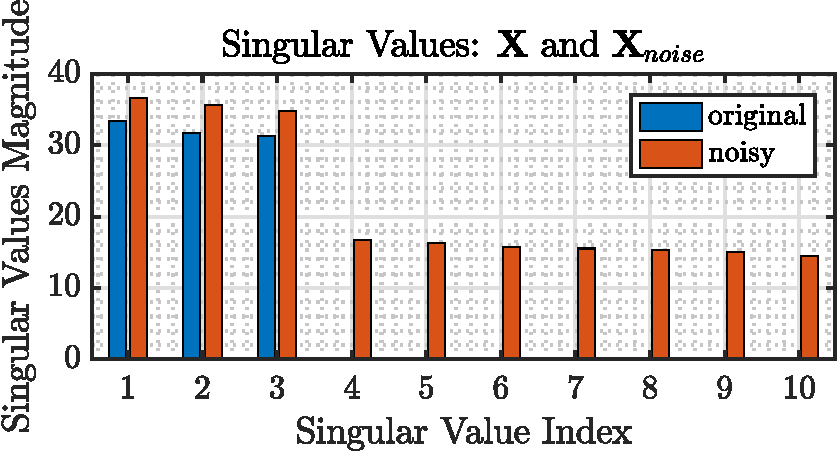
\includegraphics[height=1.5in]{report/parametric-and-line-spectra/principal-component-analysis/assets/a/svd}
    \end{subfigure}
    ~
    \begin{subfigure}{0.49\textwidth}
        \centering
        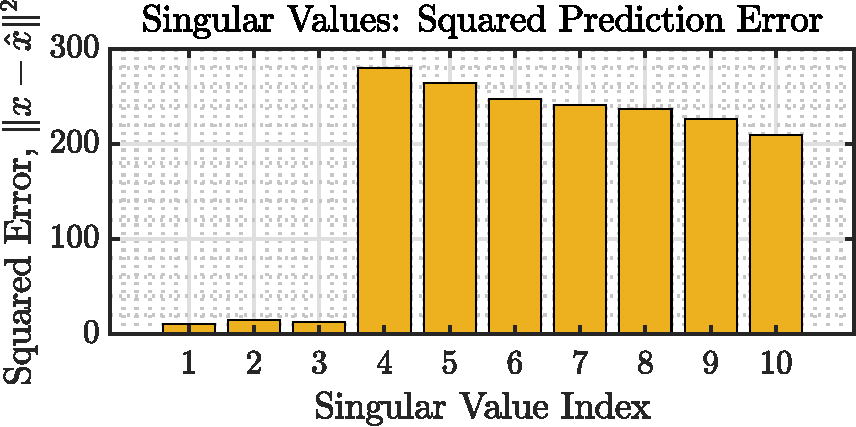
\includegraphics[height=1.5in]{report/parametric-and-line-spectra/principal-component-analysis/assets/a/error}
    \end{subfigure}
    \caption{Singular Value Decomposition: squared prediction error for corrupted signal.}
    \label{fig:2_3_a}
\end{figure}



%% b)
\item
%

Low-rank approximation of the noisy data $\mathbf{X}_{noise}$ are obtained by keeping only its $r$ most principle components.
This denoising operation relies on the assumption that the $r$ most significant components can adequately explain the data,
while the rest are pure noise. Figure \ref{fig:2_3_b} shows the approximation error
($\|\mathbf{X} - \tilde{\mathbf{X}}_{noise}\|_{F}$) for different values of $r$. Interestingly, the error is minimised
for $r = r_{true} = 3$, demostrating the power of this method, Principle Component Analysis (PCA).

\begin{figure}[h]
    \centering
    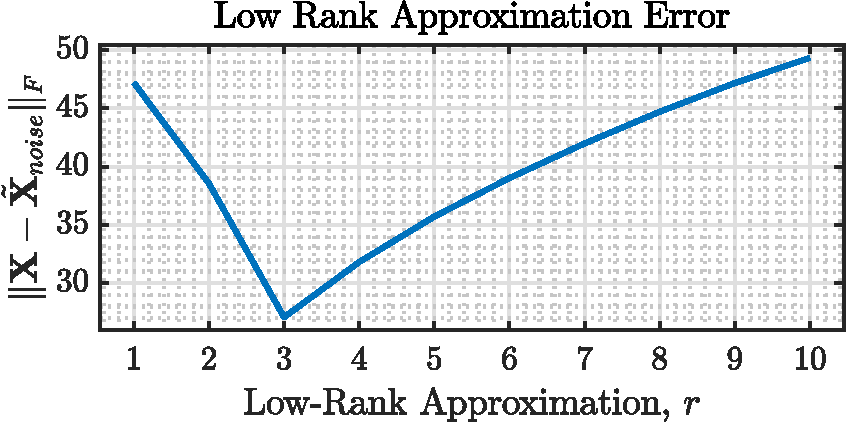
\includegraphics[height=1.5in]{report/parametric-and-line-spectra/principal-component-analysis/assets/b/low-rank_X}
    \caption{Singular Value Decomposition: squared prediction error for corrupted signal.}
    \label{fig:2_3_b}
\end{figure}

%% c)
\item
%

The parameter matrix $\mathbf{B}$ estimation is performed using OLS and PCR methods.
The estimation errors between $\mathbf{Y}$-$\mathbf{Y}_{OLS}$ and $\mathbf{Y}$-$\mathbf{Y}_{PCR}$ for the train and test datasets
are illustrated for different values of $r$ in figure \ref{fig:2_3_c}. We notice that for $r \geq 3$ the OLS and PCR methods
are score equally well at both the train and the test datasets. In more detail, while OLS performs better in training by $0.4\%$
PCR outperforms by $0.7\%$ in test set.

\begin{figure}[h]
    \centering
    \begin{subfigure}{0.49\textwidth}
        \centering
        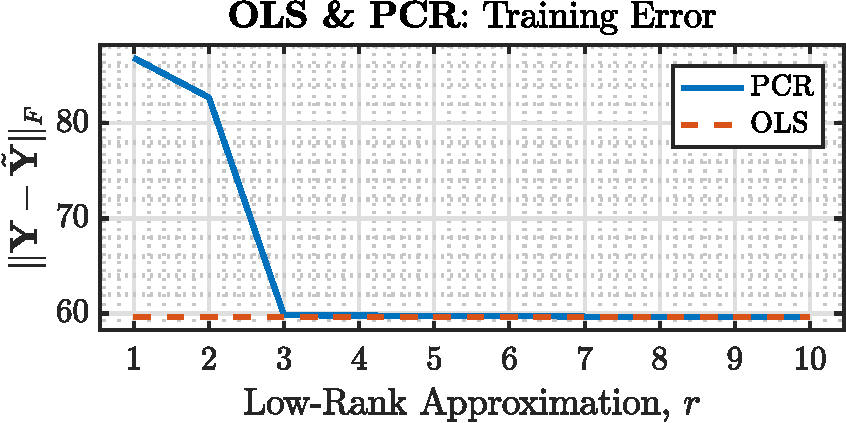
\includegraphics[height=1.5in]{report/parametric-and-line-spectra/principal-component-analysis/assets/c/ols_vs_pcr_train}
    \end{subfigure}
    ~
    \begin{subfigure}{0.49\textwidth}
        \centering
        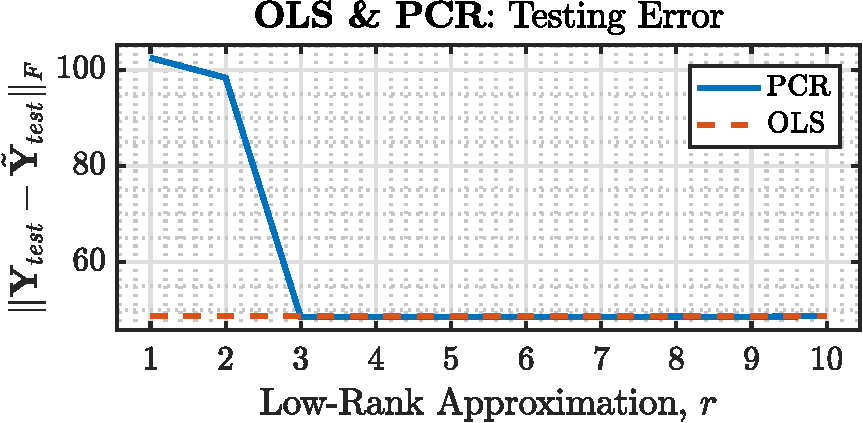
\includegraphics[height=1.5in]{report/parametric-and-line-spectra/principal-component-analysis/assets/c/ols_vs_pcr_test}
    \end{subfigure}
    \caption{Singular Value Decomposition: train \& test error.}
    \label{fig:2_3_c}
\end{figure}

%% d)
\item
%

Model evaluation of OLS and PCR models is performed over an ensemble of 100 test realisations of the stochastic process generating
$\mathbf{X}_{noise}$. Figure \ref{fig:2_3_d} summarises the prediction errors of the two models, verifying the results of the
previous part, where PCR outperforms OLS by $1.2\%$.

\begin{figure}[h]
    \centering
    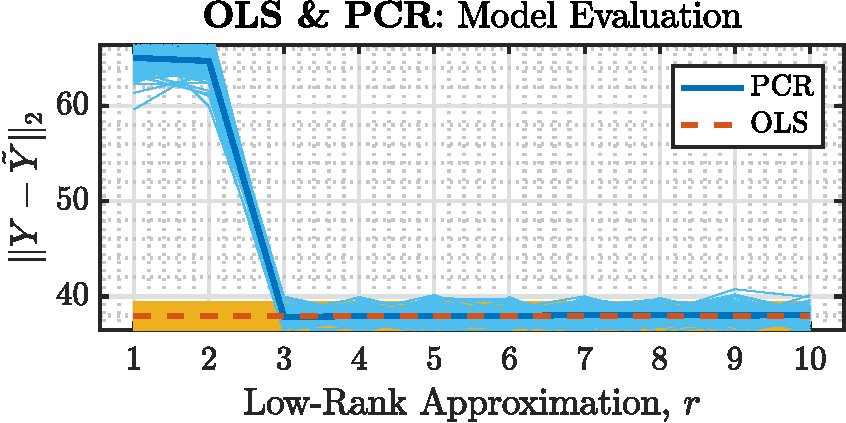
\includegraphics[height=1.5in]{report/parametric-and-line-spectra/principal-component-analysis/assets/d/regval}
    \caption{Singular Value Decomposition: model evaluation.}
    \label{fig:2_3_d}
\end{figure}

%
\end{enumerate}